\section{Order-finding}
\subsection{Problem}
This, along with the Shor's Algorithm, are one of the most useful and celebrated algorithm in the quantum computing realm till now. The problem is quite simple:  We have to find the order $r$ of a given positive integer $x$ with respect to a given $N$. The order of a number $x (<N)$ is defined as the smallest number $r$ such that
\begin{equation}
x^r = 1 (\bmod  N)
\end{equation}The above statement requires that $\gcd{(x,N)} = 1$ which can be easily checked using the Euclid's Long Division Algorithm.
\subsection{Classical Solution}
The classical solution for this problem is to compute $x^r$ for all r sequentially from  1 to $N$. This requires $O(N)$ steps and hence the time complexity is $O(N)$.
\subsection{Quantum Solution}
In this problem also like the previous ones, we get an exponential speedup. We use the quantum phase estimation we defined in the previous problem to achieve this speedup.\\
So, for the quantum case, we have two inputs: $x$ and $N$ both of which can be expressed using $L = \log(N)$ qubits. This is used to make an oracle which performs the following operation:
\begin{equation}
U|y\rangle = |xy(\bmod N)\rangle
\end{equation}where $y \in \{ 0,1 \}^L$. We have to find the eigenvectors and eigenvalues of this operator. \\
We know that $U|x^k\rangle = |x^{k+1} \bmod N \rangle$ and $U|x^{]r-1}\rangle = |1\bmod N \rangle$ where $r$ is the order. So, we will combine these various states to get our eigenvectors. So, lets say the eigenvectors are given by  
\begin{equation}
|u_s\rangle = \sum_{k=0}^{r-1} a_{k,s} |x^k \bmod N \rangle 
\end{equation}
This gives us the constraint that $a_{k-1,s} = \lambda_s a_{k,s}$ (for $k=0$, the LHS would be $a_{r-1,s}$ ) where $\lambda_s$ are the eigenvalues and hence $\lambda_s = e^{f_r(s)}$ . By simple calculations we can show that
\begin{equation}
\lambda_s = e^{2\pi is/r} \\
a_{k,s} = \frac{e^{-2\pi isk/r}}{\sqrt{r}} 
\end{equation}So the eigenvectors are 
\begin{equation}
|u_s\rangle = \frac{1}{\sqrt{r}} \sum_{k=0}^{r-1} e^{-2\pi isk/r} |x^k \bmod N \rangle 
\end{equation}Notice that the phase of eigenvalues is $s/r$. So, we can use phase estimation to get the value of $s/r$ from which we can extract $r$ with a bit of work.\\
Note that to use phase estimation we must be able to compute $U^{2^j}$. For this we use modular exponentiation. Let us say that the content of first register is$|z\rangle$ and second one is $|y\rangle$. Then the first part of phase estimation is:
\begin{equation}
\begin{split}
|z\rangle |y\rangle & \rightarrow |z\rangle U^{z_t 2^{t-1}} .... U^{z_1 2^0} |y\rangle
\\ &= |z\rangle | x^{z_t 2^{t-1}} \times ... \times x^{z_1 2^0} y (\bmod N) \rangle
\\ & = |z\rangle |x^{z} y (\bmod N) \rangle
\end{split}
\end{equation}So, we first compute the various powers of $x$ i.e. $x^{2^j} (\bmod N)$ and store them in a separate register. This can be accomplished in $O(L^3)$ steps by repeatedly squaring in $O(L^2)$ for $O(L)$ values of $j$. Then we perform the multiplication to get $x^z y (\bmod N)$ again in $O(L^3)$ steps. So, in total, this step needs $O(L^3)$ steps.\\
The other issue is that we need to have an eigenvector which depends on the order. To tackle this we give a superposition of the eigenvectors as input in the second register and as mentioned earlier this does not effect the result much and we will get a good estimate of $s/r$ for some s with great probability.\\
\begin{figure}[h]
\centering
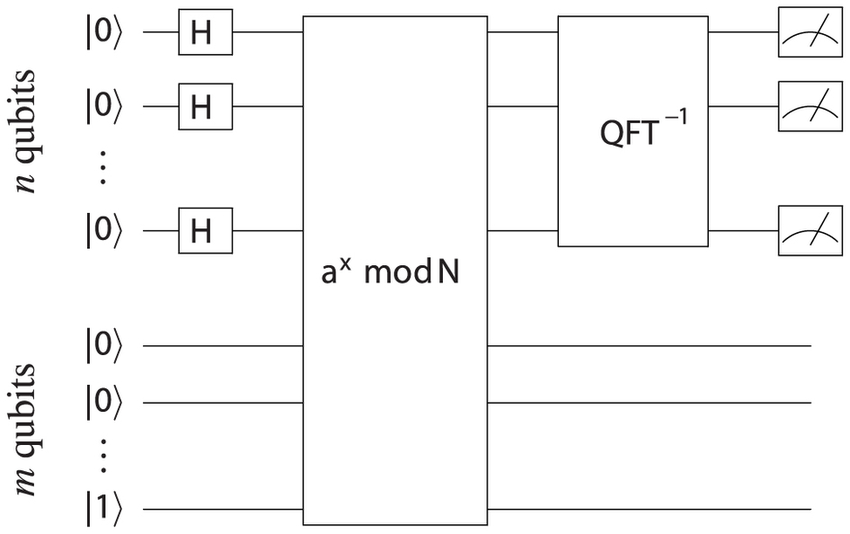
\includegraphics[width=1\textwidth]{images/order.png}
\label{order}
\caption{Circuit for finding the order. In this case we find order of  a w.r.t. N}
\end{figure}
\\To get $r$ from $s/r$ we use the method of continued fraction to obtain a good estimate of it with the error less than $1/2r^2$. Once we have approximated it, we can get a number $r'$ which will be a candidate for the order. We can easily verify if it is correct, and if it is we are done. If it is not, we will have to repeat the process again. 
\newpage
